\chapter{Marco Metodológico}
Para llevar a cabo los objetivos del proyecto se aplicó la metodología de desarrollo de software Proceso Unificado de Rational o RUP (por sus siglas en inglés) de IBM. A continuación se presentará brevemente la estructura de la metodología en cuestión, incluyendo sus fases y actividades asociadas.

\section{La metodología RUP}
El Proceso Unificado de Rational es un proceso de ingeniería de software. Provee un enfoque disciplinado hacia la asignación de tareas y responsabilidades dentro de una organización orientada al desarrollo. Su objetivo es asegurar la producción de software de alta calidad que cumpla con las necesidades de sus usuarios finales dentro de un período de tiempo y presupuesto predecibles. \cite{rupKruchten}

El Proceso Unificado de Rational captura varias de las mejores prácticas en el desarrollo de software moderno de forma que se puedan adaptar a una gama amplia de proyectos y organizaciones. Las 6 prácticas principales cubiertas por el proceso son:

\begin{enumerate}
    \item Desarrollar software iterativamente.
    \item Administrar requerimientos.
    \item Utilizar arquitecturas basadas en componentes.
    \item Modelar el software visualmente.
    \item Verificar la calidad del software.
    \item Mantener el control sobre los cambios realizados al software.
\end{enumerate}

La Figura \ref{fig:rup_iteraciones} muestra la arquitectura general del Proceso Unificado de Rational. El proceso consiste de dos dimensiones: el eje horizontal representa el tiempo y muestra los distintos ciclos de vida del software a medida que este se va desarrollando; mientras que el eje horizontal representa los principales flujos de trabajo, los cuales se encargan de agrupar actividades según su naturaleza.

Por otra parte, el eje horizontal representa el aspecto dinámico del software a medida que el proceso es aplicado. Esto se refleja en la forma de ciclos, fases, iteraciones e hitos. A su vez, el eje vertical muestra el aspecto estático del software, describiéndolo en términos de actividades, flujos de trabajo, artefactos y trabajadores.

\begin{figure}[hbt]
\begin{center}
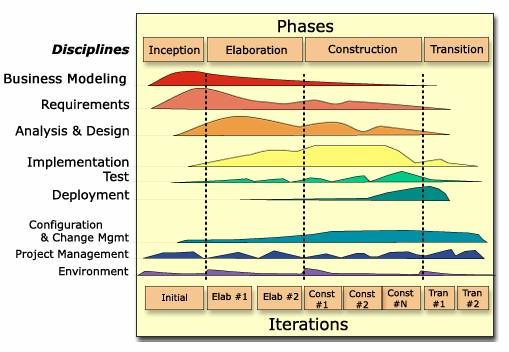
\includegraphics[scale=0.75]{./imgs/rup_iteraciones}
\caption[Iteraciones de RUP]{Arquitectura general del Proceso Unificado de Rational \cite{rupKruchten}}
\label{fig:rup_iteraciones}
\end{center}
\end{figure}

\section{Fases de RUP}
RUP divide el proceso de desarrollo de software en 4 fases. Dentro de cada una de las fases se puede realizar una cantidad variable de iteraciones dependiendo de la envergadura del proyecto. Cada fase hace hincapié en distintas actividades asociadas al desarrollo del proyecto, y producen como resultado una serie de artefactos e hitos (que deben cumplirse) con la culminación de la fase. Las fases del proceso se discuten a continuación.

\subsection{Iniciación}
La primera fase del Proceso Unificado de Rational, en la cual el ímpetu inicial para desarrollar software (una idea, un prototipo, una Solicitud de Propuesta, una evolución sobre una generación previa) se materializa hasta el punto de obtener el respaldo suficiente (al menos dentro de la organización) para poder entrar en la etapa de elaboración.

El objetivo principal de la fase de iniciación es informar y poner de acuerdo al público interesado (\textit{stakeholders}) sobre los objetivos para el ciclo de vida del proyecto. Otros objetivos de la fase incluyen:

\begin{itemize}
    \item Establecer el alcance y condiciones límite del proyecto, incluyendo el concepto de operación, criterios de aceptación y descripciones sobre lo que se desea que contenga el producto.
    \item Desarrollar los casos de uso críticos del sistema, es decir, aquellos escenarios principales que definirán la funcionalidad del producto y en los cuales se dedicará el mayor esfuerzo de desarrollo.
    \item Estimar costos, tiempos de desarrollo y costos globales para el proyecto.
\end{itemize}

Los artefactos producidos para el cierre de la fase son los siguientes:

\begin{itemize}
    \item Un documento de visión que muestre los principales requerimientos, funcionalidades y restricciones del proyecto.
    \item Un modelo de casos de uso inicial, en donde se muestre los casos de uso y actores que se pueden identificar para la fase en cuestión.
    \item Un glosario de proyecto inicial.
    \item Una propuesta de negocio inicial que incluya: el contexto del negocio, criterios de éxito y predicciones financieras.
    \item Un plan de proyecto en donde se muestren las fases (e iteraciones) a llevarse a cabo.
\end{itemize}

El hito de la fase de iniciación es la obtención y evaluación de los \textit{Objetivos de Ciclo de Vida} del proyecto. Al alcanzar este hito debe realizarse una serie de evaluaciones que deben cumplirse satisfactoriamente antes de continuar a la próxima fase del proceso. Con este hito se debe validar que las partes interesadas en el proyecto hayan llegado a un acuerdo sobre el alcance del mismo y las estimaciones de costos y tiempo. Adicionalmente, se debe validar la comprensión de los requerimientos del cliente y que estos se vean plasmados en los casos de uso principales definidos. Por último, se debe validar la credibilidad de las prioridades y riesgos asociados al proceso de desarrollo.

De todos los hitos presentes en la metodología, este es considerado como el más importante, puesto que su resultado puede llevar a la cancelación del proyecto o a un posible re-planteamiento del mismo.

\subsection{Elaboración}
Es la parte del proceso orientada a definir la visión del producto y la arquitectura a utilizar. \cite{rupKruchten} La fase de elaboración tiene como propósito analizar los problemas asociados al dominio de la aplicación, establecer una arquitectura sólida para el producto, elaborar un plan de proyecto definitivo y eliminar la mayor cantidad de elementos de alto riesgo. Cada decisión con respecto a la arquitectura del producto debe hacerse teniendo un conocimiento pleno del alcance del producto, su funcionalidad principal y requerimientos no funcionales (por ejemplo, requerimientos de desempeño).

Los objetivos principales de la fase incluyen:

\begin{itemize}
    \item Definir y validar la arquitectura del producto de la manera más rápida posible.
    \item Definir y validar la visión del proyecto.
    \item Construir un plan (de alta fidelidad) para la etapa de construcción.
    \item Demostrar que la arquitectura desarrollada puede soportar la visión por un costo y tiempo razonable.
\end{itemize}

Algunos artefactos que resultan de la ejecución de la fase son los siguientes:

\begin{itemize}
    \item Un modelo de caso de usos, completado en un 80\% como mínimo, en donde se hayan definido todos los casos de uso y actores, y se haya detallado la mayoría de los casos de uso.
    \item Una descripción definitiva de la arquitectura del software.
    \item Una lista de requerimientos suplementarios que capturen requerimientos no funcionales o aquellos que no se encuentren asociados con algún caso de uso.
    \item Una lista de riesgos y propuesta de negocio revisada.
    \item Un manual de usuario preliminar.
\end{itemize}

El hito asociado a esta fase del proceso es la \textit{Arquitectura de Ciclo de Vida}. En este hito se evalúan detalladamente los objetivos del sistema, su alcance y la arquitectura elegida. Para la aprobación del hito deben responderse, de manera favorable, una serie de preguntas, tales como: ¿la arquitectura y visión del software son estables?, ¿se han resuelto los riesgos críticos para el desarrollo del software?, ¿los gastos producidos cumplen con el presupuesto planteado? Estas preguntas, entre otras, buscan lograr un único objetivo: que el público interesado en el desarrollo, esté de acuerdo con que la visión actual puede ser alcanzada si el plan de construcción elaborado se ejecuta correctamente. Al igual que los Objetivos de Ciclo de Vida, una mala evaluación de la Arquitectura de Ciclo de Vida puede llevar a la cancelación del proyecto o a modificaciones en la visión del mismo.

\subsection{Construcción}
Es la fase del proceso en donde el software pasa del diseño arquitectónico al punto en que se vuelve un producto ejecutable que puede ser entregado a la comunidad de usuarios. \cite{rupKruchten} Durante esta fase se desarrollan todos los componentes y características del producto, se prueban meticulosamente y luego son integradas para formar un producto definitivo. La fase de construcción se caracteriza por ser la fase que contiene la mayor cantidad de actividades relacionadas con la manufactura del software, en donde se vuelve vital administrar de la mejor manera posible los recursos y actividades a ejecutar con la finalidad de optimizar costos, tiempos y calidad de producto. La fase también se puede describir como el momento en el cual el software pasa de ser una idea en la mesa de diseño a un producto tangible.

Los objetivos principales de la fase son:

\begin{itemize}
    \item Minimizar los costos de desarrollo mediante la optimización de recursos y evitando la repetición de actividades o trabajo.
    \item Alcanzar un nivel adecuado de calidad de la manera más rápida posible.
    \item Alcanzar versiones útiles del software (alfa, beta, y demás versiones de prueba) de la forma más rápida y práctica.
\end{itemize}

El resultado de la fase de construcción es un producto en condiciones para ser entregado a los usuarios finales. Los 3 artefactos que deben estar presentes para el momento de culminación son:

\begin{itemize}
    \item El producto de software, adaptado para las plataformas en donde se piensa ejecutar.
    \item Los manuales de usuario definitivos.
    \item Una descripción detallada de la versión actual del producto.
\end{itemize}

Al culminar la fase de construcción se alcanza el hito de \textit{Capacidad Operativa Inicial}. Para este hito, el equipo de desarrollo del proyecto debe decidir si el software, el entorno y los usuarios pueden entrar a un modo operativo sin exponer el proyecto a grandes riesgos. En la actualidad, dicho lanzamiento del software suele ser conocido como un lanzamiento beta. Existen 3 preguntas indispensables que deben responderse favorablemente para continuar con el proceso de desarrollo: ¿el producto cuenta con una madurez y estabilidad suficientes para ser entregado al público?, ¿el público interesado (\textit{stakeholders}) está preparado para la transición del software a los usuarios finales?, ¿los gastos generados siguen cumpliendo con el presupuesto planteado? A diferencia de los hitos de las fases anteriores, el incumplimiento favorable de la Capacidad Operativa Inicial no da como resultado la cancelación del proyecto. Los efectos desfavorables de no cumplir con el hito incluyen demoras en las fechas de lanzamiento del producto, incrementos en los gastos de producción y ejecución de iteraciones (posiblemente) no planificadas.

\subsection{Transición}
Es la cuarta fase del proceso, en donde el software es entregado a la comunidad de usuarios. \cite{rupKruchten} Cuando el producto de software se encuentra en las manos de los usuarios finales, es bastante común que surjan problemas que requieran que se corrijan errores en el código, completar funcionalidades pospuestas o crear versiones nuevas del software. La etapa de transición se inicia cuando se considera que un subconjunto de funcionalidades de la aplicación ha sido completado con un nivel aceptable de calidad y existe suficiente documentación que permita que el usuario pueda producir buenos resultados al interactuar con el producto. La fase incluye las siguientes actividades:

\begin{itemize}
    \item Pruebas del producto beta para validar el producto nuevo frente las expectativas de los usuarios.
    \item Operación en paralelo del producto nuevo con la aplicación que se desea sustituir.
    \item Conversión de bases de datos operativas.
    \item Entrenamiento de usuarios y personal de mantenimiento.
    \item Entrega del producto de software a los equipos de mercadeo, distribución y ventas.
\end{itemize}

Los principales objetivos de la fase son:

\begin{itemize}
    \item Lograr que el usuario se familiarice con el producto y pueda utilizarlo de forma autónoma.
    \item Lograr que el público interesado en el proyecto otorgue el visto bueno sobre la culminación del desarrollo.
    \item Lograr un producto final de forma rápida y rentable.
\end{itemize}

Al finalizar la fase de transición se obtiene el último hito perteneciente al proceso, el \textit{Lanzamiento del Producto}. En este momento el público interesado, en especial el equipo desarrollador, debe decidir si los objetivos del proyecto (definidos en los Objetivos de Ciclo de Vida) se han cumplido y si es necesario iniciar un nuevo ciclo de vida. Las principales interrogantes a responder para la aceptación del hito son: ¿el usuario final se encuentra satisfecho con el producto?, ¿los gastos totales cumplieron con los gastos presupuestados?

Una particularidad interesante de la fase de transición es que alcanzar esta fase suele ser un buen augurio para el producto. Por lo tanto, es bastante común en las empresas de software tomar una decisión temprana sobre el comienzo de un ciclo de vida nuevo para el producto. Por lo tanto, es común observar que una fase de transición de un producto va acompañada de una ejecución en paralelo de una fase de iniciación para un nuevo lanzamiento del producto.

\section{Fases contempladas para el proyecto}
